
\documentclass[tikz,border=4pt]{standalone}
\usepackage{tikz}
\usepackage{amsmath}
\usepackage{amssymb}
\usetikzlibrary{arrows.meta,positioning,fit,backgrounds,shapes.geometric,
                decorations.pathreplacing,calc,shadows.blur,shapes.arrows}

% ------------------------------------------------------------------
% Color palette (muted, print-safe, AAAI-friendly)
% ------------------------------------------------------------------
\definecolor{frozenblue}{RGB}{54,89,150}
\definecolor{frozenbluefill}{RGB}{223,232,246}
\definecolor{loraorange}{RGB}{196,110,32}
\definecolor{lorafill}{RGB}{250,231,213}
\definecolor{tourgreen}{RGB}{60,110,70}
\definecolor{tourfill}{RGB}{222,236,222}
\definecolor{selpurple}{RGB}{104,72,140}
\definecolor{selfill}{RGB}{233,224,242}
\definecolor{neutralgray}{RGB}{90,90,90}
\definecolor{neutralfill}{RGB}{240,240,240}

\tikzset{
  frozenbox/.style={rectangle, rounded corners=2pt, draw=frozenblue, thick,
    fill=frozenbluefill, minimum width=2.6cm, minimum height=1.05cm,
    align=center, font=\scriptsize},
  lorabox/.style={rectangle, rounded corners=2pt, draw=loraorange, thick,
    fill=lorafill, minimum width=2.6cm, minimum height=1.05cm,
    align=center, font=\scriptsize},
  tourbox/.style={rectangle, rounded corners=2pt, draw=tourgreen, thick,
    fill=tourfill, minimum width=2.9cm, minimum height=1.15cm,
    align=center, font=\scriptsize},
  selbox/.style={rectangle, rounded corners=2pt, draw=selpurple, thick,
    fill=selfill, minimum width=2.9cm, minimum height=1.15cm,
    align=center, font=\scriptsize},
  databox/.style={rectangle, rounded corners=1pt, draw=neutralgray,
    fill=neutralfill, minimum width=2.2cm, minimum height=0.85cm,
    align=center, font=\scriptsize},
  decision/.style={diamond, draw=selpurple, thick, fill=selfill, aspect=2.4,
    align=center, font=\scriptsize, inner sep=1pt},
  flow/.style={-{Stealth[length=2mm]}, thick, draw=neutralgray},
  loopflow/.style={-{Stealth[length=2mm]}, thick, draw=neutralgray, dashed},
  groupbg/.style={rounded corners=6pt, draw=none, fill=black!4},
  lockicon/.style={font=\scriptsize\bfseries, frozenblue}
}

\begin{document}
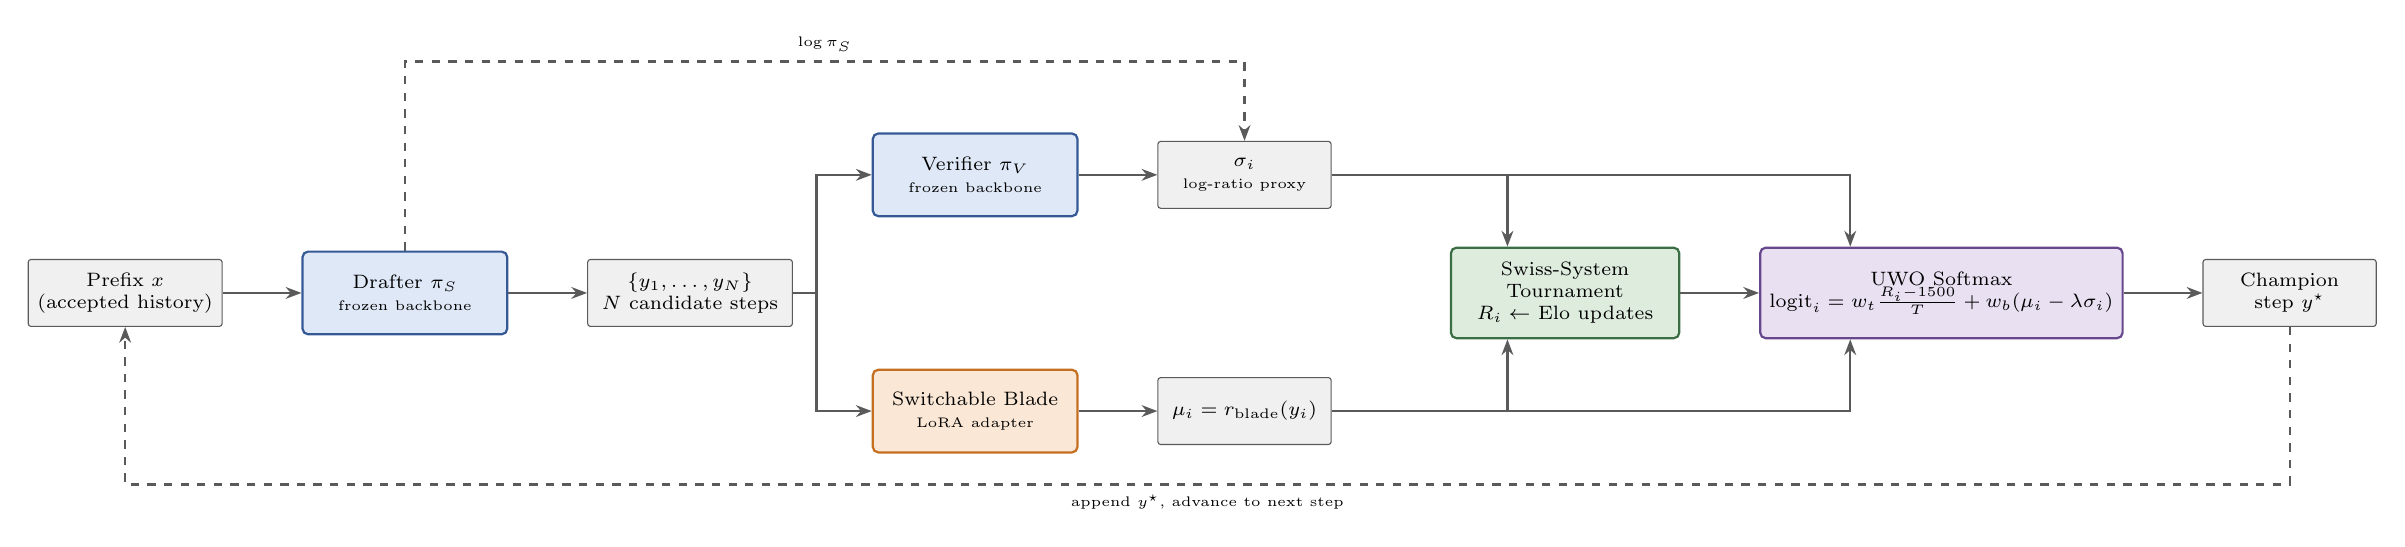
\begin{tikzpicture}[node distance=8mm and 10mm]

  % --- input ---
  \node[databox] (prefix) {Prefix $x$\\ \scriptsize(accepted history)};

  % --- drafting ---
  \node[frozenbox, right=of prefix] (drafter) {Drafter $\pi_S$\\ \tiny frozen backbone};
  \node[databox, right=of drafter, minimum width=2.6cm] (cands)
       {$\{y_1,\dots,y_N\}$\\ \scriptsize $N$ candidate steps};

  % --- scoring ---
  \node[frozenbox, right=10mm of cands, yshift=15mm] (verifier) {Verifier $\pi_V$\\ \tiny frozen backbone};
  \node[lorabox, right=10mm of cands, yshift=-15mm] (blade) {Switchable Blade\\ \tiny LoRA adapter};

  \node[databox, right=10mm of verifier] (sigma) {$\sigma_i$\\ \tiny log-ratio proxy};
  \node[databox, right=10mm of blade] (mu) {$\mu_i = r_{\mathrm{blade}}(y_i)$};

  % --- tournament ---
  \node[tourbox, right=15mm of sigma, yshift=-15mm] (tour)
       {Swiss-System\\ Tournament\\ \scriptsize $R_i \leftarrow$ Elo updates};

  % --- selection ---
  \node[selbox, right=10mm of tour] (uwo)
       {UWO Softmax\\ \scriptsize $\mathrm{logit}_i = w_t\frac{R_i-1500}{T} + w_b(\mu_i-\lambda\sigma_i)$};

  % --- outputs ---
  \node[databox, right=10mm of uwo] (champ) {Champion\\ step $y^\star$};

  % ---------------- edges ----------------
  \draw[flow] (prefix) -- (drafter);
  \draw[flow] (drafter) -- (cands);
  
  \draw[flow] (cands.east) -- ++(3mm,0) |- (verifier.west);
  \draw[flow] (cands.east) -- ++(3mm,0) |- (blade.west);
  
  \draw[flow] (verifier) -- (sigma);
  \draw[flow] (blade) -- (mu);
  
  % drafter to sigma (dashed) for log-ratio proxy
  \draw[flow, dashed] (drafter.north) -- ++(0, 24mm) -| (sigma.north)
        node[pos=0.25, above, font=\tiny]{$\log \pi_S$};
  
  % mu and sigma to tour
  \draw[flow] (sigma.east) -| ($(tour.north)!0.5!(tour.north west)$);
  \draw[flow] (mu.east) -| ($(tour.south)!0.5!(tour.south west)$);
  
  \draw[flow] (tour) -- (uwo);
  
  % mu and sigma to uwo (bypassing tour)
  \draw[flow] (sigma.east) -| ($(uwo.north)!0.5!(uwo.north west)$);
  \draw[flow] (mu.east) -| ($(uwo.south)!0.5!(uwo.south west)$);
  
  \draw[flow] (uwo) -- (champ);
  
  % loop back
  \draw[loopflow] (champ.south) -- ++(0,-20mm) -| (prefix.south)
        node[pos=0.25, below, font=\tiny]{append $y^\star$, advance to next step};

\end{tikzpicture}
\end{document}
